\section{Testvorbereitung}
Wir w�hlen die InnoDB als Speichermaschine aus, da sie die Transaktionssicherheit gew�hrleistet und sich dadurch f�r das Betreiben eines Webshops am besten eignet. 
Jede Versuchsreihe entspricht einer bestimmten Konfiguration und besteht aus vier Testl�ufen zu je einem Use Case. Am Anfang  werden Testdaten mit einer  bestimmten Anzahl von Kunden, einer konstanten Anzahl von Produkten (1000), einer konstanten Anzahl von Warenk�rben pro Kunde(5) und genauso einer konstanten Anzahl von Produkten pro Warenkorb(5) generiert. Die Anzahl der Kunden erh�ht sich mit jedem Testlauf. In jeder Versuchsreihe werden die vier verschiedenen Use Cases betrachtet, die durch eine unterschiedliche SELECT-Anweisung an die MySQL-Datenbank realisiert werden:
\subsection{SELECT-Anweisungen}
\begin{enumerate}
\item \textbf{Use Case 1: Welches Produkt wurde wie oft gekauft?}
\lstset{language=Java,caption={UseCase1},label=Use Case 1}
\lstinputlisting[language=Java]{Christof/Listings/UseCase1.java}
\item \textbf{Wieviel Umsatz wurde von wem in bestimmtem Zeitraum generiert?}
\lstset{language=Java,caption={UseCase2},label=Use Case 2}
\lstinputlisting[language=Java]{Christof/Listings/UseCase2.java}
\item \textbf{Wie viele Kunden haben in bestimmten Zeitraum bestellt?}
\lstset{language=Java,caption={UseCase3},label=Use Case 3}
\lstinputlisting[language=Java]{Christof/Listings/UseCase2.java}
\item \textbf{Wie viel Umsatz wurde an den ersten drei Tagen der ersten drei Monate generiert?}
\lstset{language=Java,caption={UseCase4},label=Use Case 4}
\lstinputlisting[language=Java]{Christof/Listings/UseCase2.java}
\end{enumerate}

\subsection{Konfigurationen der MySQL-Datenbank und der Tabellen}
Jede Versuchsreihe testet die SELECT-Anweisungen mit einer bestimmten Konfiguration der MySQL-Datenbank und der Tabellen. Vor jedem Testlauf werden die entsprechenden Konfigurationseintellungen mit SQL-Anweisungen durchgef�hrt.
\begin{enumerate}
\item \textbf{K1} : Kaltstart ohne Index
\item \textbf{K2} : Warmstart ohne Index
\item \textbf{K3} : Hash-Indizes auf Primary Keys und Foreign Keys / ohne Partitioning
\item \textbf{K4} : B-Tree-Indizes auf Primary Keys und Foreign Keys / ohne Partitioning
\item \textbf{K5} : Hash-Indizes auf Primary Keys und Foreign Keys sowie B-Tree-Index auf Datum / ohne Partitioning
\item \textbf{K6} : Hash-Indizes auf Primary Keys und Foreign Keys sowie B-Tree-Index auf Datum / mit List-Partitioning auf MONTH(Datum) f�r jedes Quartal
\item \textbf{K7} : Hash-Indizes auf Primary Keys und Foreign Keys sowie B-Tree-Index auf Datum / mit Hash-Partitioning auf MONTH(Datum) f�r jeden Monat
\item \textbf{K8} : Hash-Indizes auf Primary Keys und Foreign Keys sowie B-Tree Index auf Datum / mit Range-Partitioning auf COLUMNS(Datum) f�r jedes Quartal
\item \textbf{K9} : Hash Indizes auf Primary Keys und Foreign Keys sowie B-Tree-Index auf Datum / mit Sub-Partitioning (Range-Partitioning quartalsweise auf Datum und f�r jedes Quartal jeweils vier Hash-Partitions auf TO\_DAYS(Datum))
\item \textbf{K10}: Hash-Indizes auf Primary Keys und Foreign Keys / mit Sub-Partitioning (Range-Partitioning quartalsweise auf Datum und f�r jedes Quartal jeweils vier Hash-Partitions auf TO\_DAYS(Datum)
\end{enumerate}

\subsection{EXPLAIN-Anweisung}
Bei den SQL-Abfragen stellten wir bei jeder SELECT-Anweisung ein EXPLAIN davor, um n�tzliche Informationen zum Ausf�hrungsplan des Optimierers zu erhalten. Die EXPLAIN-Anweisung liefert u.a. Daten dar�ber, ob die Indizes auch wirklich benutzt wurden, in welcher Reihenfolge die Tabellen verkn�pft werden sowie weitere Informationen, die helfen sollen die SELECT-Anweisungen zu beschleunigen.  
\subsection{EXPLAIN PARTITIONS-Anweisung}
Diese Anweisung liefert zus�tzlich Informationen �ber die verwendeten Partitionen. Man kann sie jedoch nur auf RANGE- oder LIST-partitionierte Tabellen verwenden. Bei KEY- oder HASH-Partitionen ist sie unbrauchbar, da automatisch alle Partitionen ausgegeben werden. 

\section{Testdurchf�hrung}

\subsection{Annahmen und Vor�berlegungen}
\begin{enumerate}
\item Der Warmstart ohne Index(K2) sollte gegen�ber einem Kaltstart ohne Index(K1) eine Geschwindigkeitssteigerung bewirken, da die Queries und deren Ergebnismenge durch die vorherige Abfrage in Query-Cache gespeichert wurden.
\item Das Hinzuf�gen von Indizes ist der erste wichtige Schritt bei der Optimierung von SELECT-Anweisungen und sollte bei der richtigen Formulierung der SELECT-Anweisung einen enormen Geschwindigkeitsvorteil gegen�ber Abfragen auf Tabellen ohne Indizes bieten. Es ist die Frage zu beantworten, ob es bei diesen Use Cases einen gro�en Geschwindigkeitsunterschied zwischen der Hash-Indizierung(K3) und der B-Tree-Indizierung(K4) gibt und wodurch sich eventuelle Unterschiede ergeben.  
\item Wenn wir die Konfiguration K3 nehmen und diese um ein B-Tree-Index auf das Datum(K5) erg�nzen, sollten bei dem Use Case 3 die Zeilen mit dem gesuchten Datum schneller gefunden werden als ohne den B-Tree-Index.
\item Eine zus�tzliche List-Partitionierung auf die drei Monate in jedem Quartal sollte die Suche nach einem konstanten Datumswert(Use Case 3) noch schneller ablaufen, denn es wird nur in der einen Partition gesucht.          \item (--------------wird noch erg�nzt---------------)
\item usw.
\end{enumerate}
\subsection{Testergebnisse bei einer Million Kunden}

\begin{figure}[htp]
\centering
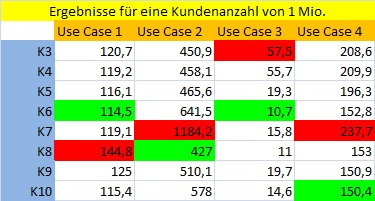
\includegraphics[width=0.75\textwidth]{Christof/Bilder/auswert1.jpg}
\caption{Testergebnisse}
\label{fig:auswert1}
\end{figure}

\subsection{Testauswertung}
\begin{enumerate}
\item Der Kaltstart ohne Index(K1) gegen�ber dem Warmstart ohne Index(K2) hat keinen Geschwindigkeitsvorteil gebracht. Die Werte unterscheiden sich nur sehr gering voneinander. Wahrscheinlich liegt es an der geringen Komplexit�t der Statements und der kleinen Anzahl von Tabellen, da das Parsen dadurch nicht viel zeitaufw�ndiger ist.
\item Die Indizes brachten wie erwartet einen enormen Geschwindigkeisunterschied, bei 100 Tausend Kunden hat die Abfrage f�r den Use Case 1 um den Faktor 29 k�rzer gedauert. Im direkten Vergleich zwischen K3 und K4 gab es so gut wie keine Unterschiede bei allen Use Cases. Auch der Ausf�hrungsplan mit Hilfe der EXPLAIN-Anweisung zeigte keine Unterschiede bei den Zugriffstypen. Bei allen Use Cases wurde auf die selbe Art auf die Tabellen zugegriffen.    
\item Die Vermutung hat sich best�tigt und bei dem Use Case 3 gibt es eine deutliche Performancesteigerung mit dem zus�tzlichen B-Tree-Index auf das Datum(K5). Es bleibt nun aber die Frage zu kl�ren, wieso sich der Use Case 2 bei dieser Konfiguration als einziger verschlechtert hat obwohl die Zugriffstypen im Vergleich zur Konfiguration 3 die selben sind und die B-Tree-Indizierung f�r BETWEEN-Operatoren eigentlich gut geeignet ist.
\item Der Use Case 3 ist mit der Konfiguration 6 tats�chlich noch schneller ausgef�hrt worden, was haupts�chlich an dem List-Partitioning liest. Die Zeit f�r den Use Case 2 hat sich jedoch noch weiter verschlechtet.
\item (--------------wird noch erg�nzt---------------) 
\item (--------------wird noch erg�nzt---------------)
\item usw.      
\end{enumerate}

\subsection{Alle Messwerte}
\begin{figure}[htp]
\centering
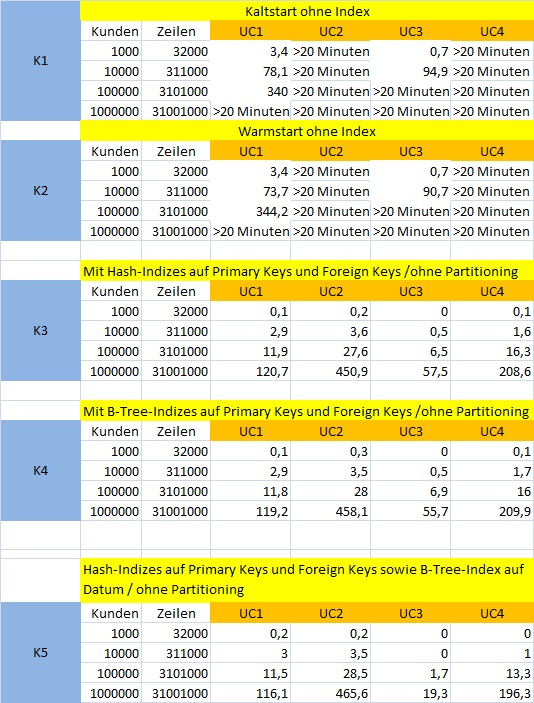
\includegraphics[width=1\textwidth]{Christof/Bilder/TabTeil1.jpg}
\caption{Messwerte Teil 1}
\label{fig:erg1}
\end{figure}

\begin{figure}[htp]
\centering
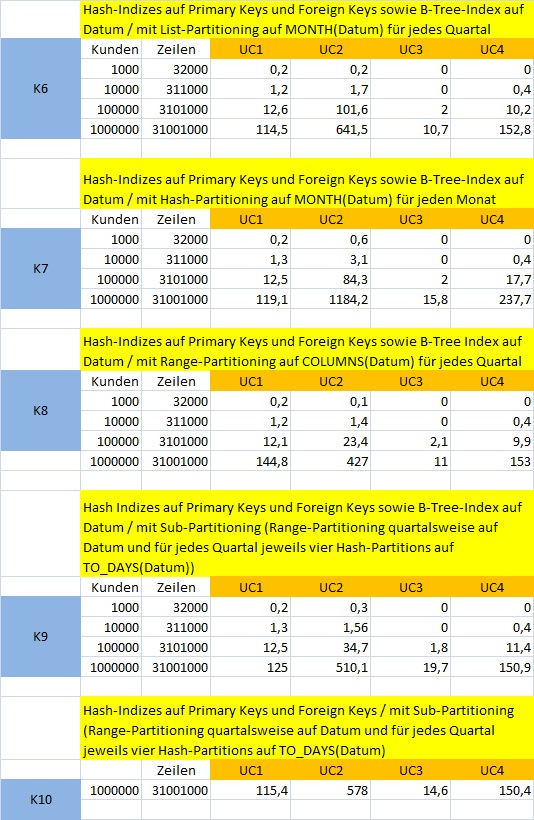
\includegraphics[width=1\textwidth]{Christof/Bilder/TabTeil2.jpg}
\caption{Messwerte Teil 2}
\label{fig:erg2}
\end{figure}



